\section{Background}
\label{sec:background}

\textbf{Single-Instruction Multiple-Data} (SIMD) parallelism is available on modern processors through vector units.
The vector instructions executed in these units encode operations to be performed on vector registers.
Each data item in a vector register occupies a \emph{vector lane}, or \emph{lane}.
The \textbf{length  of vector} (VL) is the number of bits in a vector register, while the number of data items in a vector register is the \textbf{vector factor} (VF).
Traditionally, VL was a constant known at compilation time, however novel \textbf{Instruction-Set Architecture} (ISAs) have vector-length agnostic vector instructions where the VL is not known at compilation time --- and can even be changed at runtime by the hypervisor.
An example of such a design is the Arm \textbf{Scalable Vector Extensions} (SVE) available on ARM v8.3 \& v9 processors and Fujitsu's A64FX\footnote{At the time of writing, A64FX is the only available processor that supports SVE.}.
Vector units may also have \emph{predicate vectors}, 
 which are bit-vector registers where each bit indicates if a corresponding lane of the vector register is \emph{active}.
Instructions that accept predicate registers are known as \emph{predicated instructions}, and they only operate on active lanes --- inactive lanes are left unchanged.
Predicated instructions can be used to enable the vectorization of loops that contain control-flow instructions.

\begin{center}
\begin{minipage}[t]{0.8\columnwidth}
\begin{lstlisting}[
escapechar=|,
language=C,
caption={A control-flow divergent loop.}, label=lst:simple-loop]
for (i = 0; i < n; i++) {
    if (a[i] < b[i]) { |\label{lst:simple-loop:condition}|
        a[i] = b[i] * c[i]; |\label{lst:simple-loop:true-path}|
    } else{
        b[i] = a[i] + c[i]; |\label{lst:simple-loop:false-path}|
    }
}
\end{lstlisting}
\end{minipage}
\end{center}

\iffalse
\begin{lstlisting}[
escapechar=|,
language=C,
caption={\rlst{simple-loop}'s loop after control-flow linearization.}, label=lst:predicated-loop]
for (i = 0; i < n; i++) {
    pred_t = a[i] < b[i]; |\label{lst:predicated-loop:pred-true}|
    pred_f = ! pred_t; |\label{lst:predicated-loop:pred-false}|
    [[ pred_t ]] a[i] = b[i] * c[i]; |\label{lst:predicated-loop:true-path}|
    [[ pred_f ]] b[i] = a[i] + c[i]; |\label{lst:predicated-loop:false-path}|
}
\end{lstlisting}

\begin{lstlisting}[
escapechar=|,
language=C,
caption={\rlst{predicated-loop}'s loop after vectorization.}, label=lst:vectorized-loop]
for (i = 0; i < n; i+=VL) {
    pred_t = a[i:i+VL] < b[i:i+VL]; |\label{lst:vectorized-loop:pred-true}|
    pred_f = ! pred_t; |\label{lst:vectorize-loop:pred-false}|
    [[ pred_t ]] a[i:i+VL] = b[i:i+VL] * c[i:i+VL]; |\label{lst:vectorized-loop:true-path}|
    [[ pred_f ]] b[i:i+VL] = a[i:i+VL] + c[i:i+VL]; |\label{lst:vectorized-loop:false-path}|
}
\end{lstlisting}
\fi

\begin{figure}
     \centering
     \begin{subfigure}[b]{0.3225\columnwidth}
         \centering
         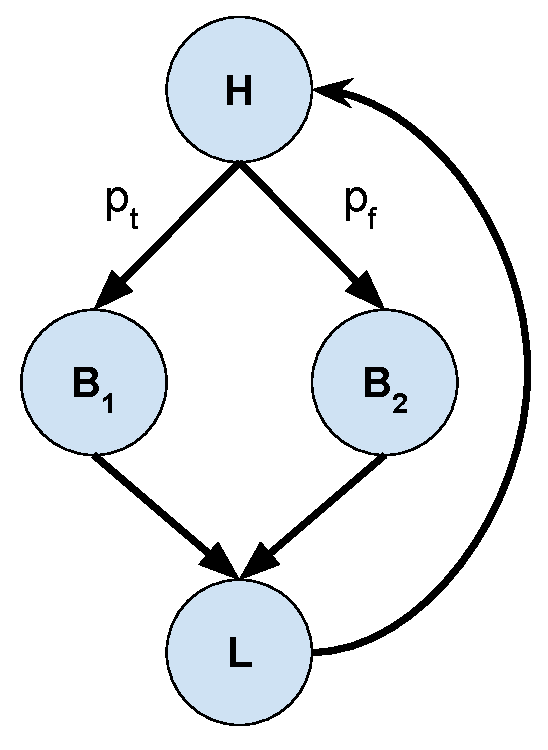
\includegraphics[width=\textwidth]{Figures/02-background/simple-loop-cfg.pdf}
         \caption{Original.}
         \label{fig:simple-loop-cfg}
     \end{subfigure}
     \begin{subfigure}[b]{0.25\columnwidth}
         \centering
         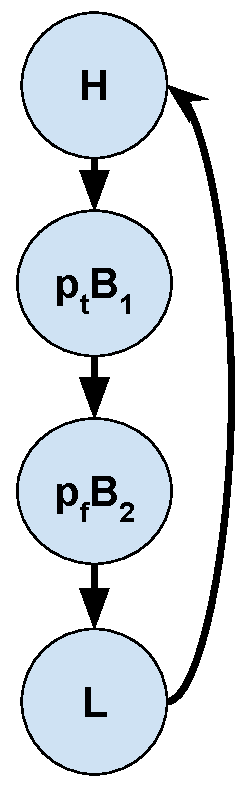
\includegraphics[height=0.17\textheight]{Figures/02-background/simple-loop-predicated-cfg.pdf}
         \caption{Linearized.}
         \label{fig:simple-loop-predicated-cfg}
     \end{subfigure}
     \begin{subfigure}[b]{0.3225\columnwidth}
         \centering
         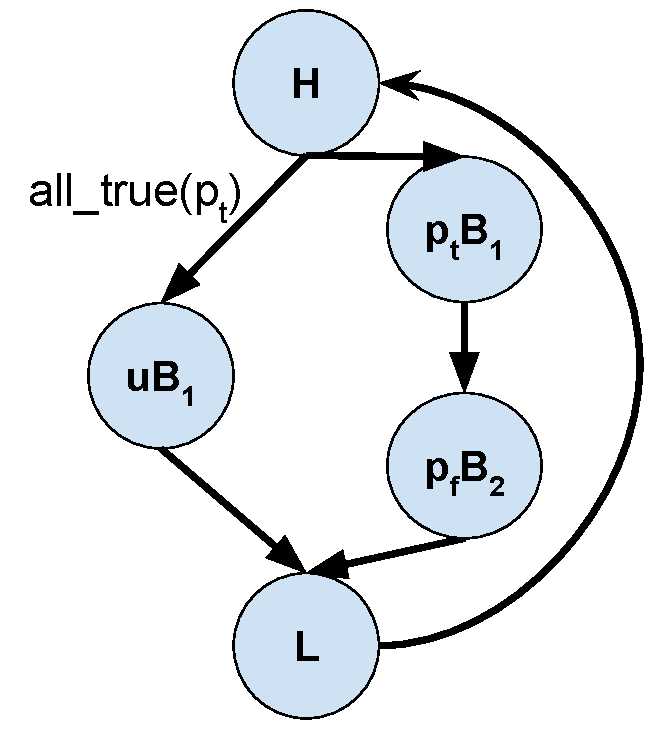
\includegraphics[height=0.17\textheight]{Figures/02-background/simple-loop-bossc-cfg.pdf}
         \caption{BOSCC.}
         \label{fig:simple-loop-boscc-cfg}
     \end{subfigure}
        \caption{(a) Original CFG of \rlst{simple-loop}; (b) CFG after control-flow linearization (CFL); (c) CFG in (b) after inserting of \code{all\_true} BOSCC.}
        \label{fig:simple-loop-cfgs}
\end{figure}

In a loop with \emph{divergent} control flow,  different iterations of the loop may execute instructions from different paths in the loop's \textbf{Control-Flow Graph} (CFG).
Divergent control flow may be an obstacle to the vectorization of a loop.
Common constructs in computer code, such as \code{if-then-else} and \code{switch-case} statements may introduce divergence.
Modern compilers are able to vectorize some control-flow divergent loops after applying a \textbf{Control-Flow Linearization} (CFL) technique known as \code{If}-Conversion.
If conversion transforms control-flow dependencies into data dependencies \cite{allen_conversion_1983, park1991ifconversion}.
For instance, consider the \code{for}-loop in \rlst{simple-loop} and its CFG in \rfig{simple-loop-cfg}.
The statements on \rline{simple-loop:true-path} and \rline{simple-loop:false-path} are control-flow dependent on the condition in \rline{simple-loop:condition}.
CFL eliminates control flow by first computing a predicate register for each possible path.
Then the instructions on each basic block are predicated with the predicate registers that correspond to the condition that needs to be true for that block to be executed.
For example, instructions in block $B_1$ are predicated with a predicate register $p_t$, where $p_t = (a[i] < b[i])$.
$B_2$ are predicated with a predicate register $p_f$, where $p_f = (a[i] \leq b[i]) = \neg p_t$.
\rfig{simple-loop-predicated-cfg} shows the CFG in \rfig{simple-loop-cfg} after CFL, where predicated blocks are denoted by prefixing the original block name with their corresponding predicate register.

Once the body of a loop is linearized via CFL, vectorization proceeds with the conventional recipe followed by most modern compilers, which consists in widening scalar operands into vector operands and replacing scalar operations with their equivalent vector versions.
Scalar predicate registers are replaced with vector predicate registers.
Predicated execution, or simply \emph{predication}, of scalar instructions is supported on modern processors via predicated instructions.
For vector instructions, predication is supported via predicated vector instructions or bit-wise vector instructions, in a process known as \emph{masking}.

Although CFL enables the use of SIMD instructions, it clearly wastes resources and computational cycles because all instructions from each mutually exclusive path will be executed but only one path will have their computations committed.
Generating \textbf{Branch-On-Superword-Condition-Codes} (BOSCCs) is a common technique to avoid executing instructions from paths where vector lanes would be inactive \cite{ jaewook_shin_superword-level_2005, shin_introducing_2007, shin_evaluating_2009}.
BOSCCs are instructions, or a sequence of instructions, that dynamically checks the uniformity of predicate registers.
In a uniform predicate register the condition evaluates to the same value --- all true or all false --- for all lanes.
In such cases, only the instructions corresponding \emph{uniform path}, true path or false path, need to be executed.
For example, after vectorization, in \rfig{simple-loop-predicated-cfg} if $p_t$ is a uniform true vector, then only instructions in $B_1$ need to be executed and instructions in $B_2$ can be skipped.
\rfig{simple-loop-boscc-cfg} shows the CFG in \rfig{simple-loop-predicated-cfg} after BOSCCs are inserted by the compiler.
As \rfig{simple-loop-boscc-cfg} shows, an \code{all\_true} \emph{guard condition} is generated to check if $p_t$ is a uniform true vector.
In such a case, the control flow is directed to a uniform block $uB_1$, that only contains instructions from block $B_1$.
When $p_t$ is a uniform true vector, the instructions in block $B_2$ can be skipped because $p_f = \neg p_t$, and thus all lanes would be inactive.

The insertion of BOSCCs can improve SIMD utilization and reduce the number of wasted cycles by avoiding executing vector instructions with all lanes inactive.
However, the benefits of BOSCCs can only be observed if uniform vectors occur frequently.
If uniformity is rare, then the use of BOSCCs does not increase SIMD utilization \cite{praharenka_vectorizing_2022}.
Moreover, the likelihood of uniformity decreases with increased VL, thus uniform predicate vectors are less likely to be found for architecture with long vectors --- e.g. AVX512, Fujitsu A64Fx.
\textbf{Active-Lane Consolidation} (ACL) is an algorithm proposed to increase SIMD utilization even in the presence of infrequent uniform vectors and architectures with long vectors \cite{praharenka_vectorizing_2022}.
At the core, ACL is a permutation algorithm that creates uniform vectors by merging active lanes from two, or more, non-uniform vectors into a \emph{merged vector}.
Permutation enables ALC to only execute non-predicated blocks with the constructed uniform vector and effectively avoid executing linearized code.

Praharenka \etal propose ALC as an algorithm and manually apply it to each evaluated benchmark.
This work shows presents the first compiler-only optimization pass that automatically applies ALC to a loop that contains divergent control flow. 
Furthermore, during the seminal work of Praharenka \etal they had no access to a processor that implements SVE.
Therefore, all their experimental results are based on simulations conducted with the Arm's Instruction Emulator (ArmIE).
Therefore, Praharenka \etal's work only shows improvements in terms of the reduction in the number of executed instructions.
Our performance study on a hardware implementation of SVE revealed that some of the estimates for the latency of instructions used by Praharenka \etal were significantly off.
This work shows that accounting for the actual instruction latencies in a hardware implementation of ALC requires a redesign of aspects of ALC
To the best of our knowledge, this work is the first to show ALC's performance on real hardware.
Moreover, it identified limitations on the original algorithm that will be discussed in the following section.

\iffalse
% ######  ATTENTION #############
% The content bellow was left as a reference and is not going to be used for the paper.
% ######  ATTENTION #############
\subsection{If-Coversion}

A traditional vectorization pass in a compiler consists in performing a legality check and a cost analysis, unrolling a loop, and then simply replacing a set of scalar instructions with vector ones.
In some traditional vectorization passes, if the loop contains control-flow instructions, the legality check fails because in a loop that may exhibit control-flow divergence (e.g., if-then-else or switch-case statements) different iterations of the loop can take different paths.

If-Conversion is a well-known compiler transformation that tries to solve this problem by utilizing \emph{predicated instructions}. 
Predicated instructions are a set of instructions guarded by a one-bit predicate. Instructions with a true predicate are executed while instructions guarded by a false predicate are treated as no-operation by the processor.

In a processor with \emph{predicated Vector instructions}, compilers can vectorize divergent loops by first linearizing control flow and then replacing scalar instructions with vectorized ones.

\begin{figure*}[h]
  \centering
  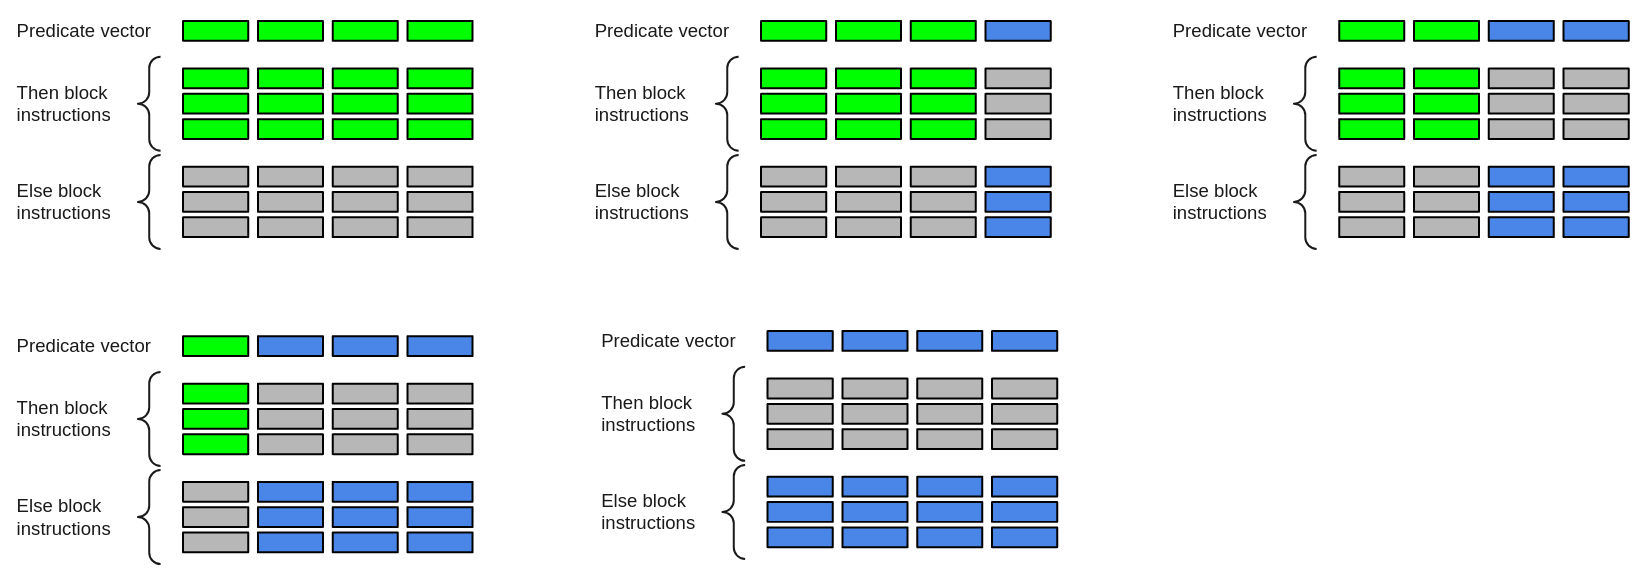
\includegraphics[width=\textwidth]{Figures/condition_distribution.png}
  \caption{Wasting vector lanes due to predication}
\end{figure*}

\begin{lstlisting}[language=C, caption={If-Converted Code}]
    VLength= 4;
    for(i = 0; i < n; i+=VLength ){
        a_v = load_v(&a[i], VLength);
        b_v = load_v(&b[i], VLength);
        c_v = load_v(&c[i], VLength);
        mask_v = load_v(&cond[i], VLength);
        mask_not_v = not_v(mask_v);
        mult_v = masked_mul(b_v, c_v, mask_v);
        masked_store_v(&a[i], mult_v, VLength, mask_v);
        add_v = maked_add(a_v, b_v, mask_v);
        masked_store_v(&b[i],add_v, VLength, mask_not_v);
    }
\end{lstlisting}


Listing 1 contains a simple loop with an if-then-else statement where the if condition depends on the loop index variable. 
Thus, different iterations of the loop may take different paths. 
\nelson{I do not see listing 2 with the vectorized code in the generated pdf.}
The corresponding vectorized code is shown in Listing 2 assuming that the vector length is 4. 
An efficient code generation strives to reduce the number of predicated instructions used due to their overheads.
Thus, a solution is to load all the lanes of the vectors without predication, and then create the predicate vectors.  
The arithmetic computations are also done without predication, and the storing of the results is predicated. 


\subsection{Branch on Super-Word Condition-Codes (BOSCCs)}
an issue with If-conversion is that half of vector lanes are wasted due to predication when code is always executed for both the if and the else blocks

\nelson{I do not see a figure with green and blue elements. BTW green and blue are bad choices for people that are color blind.}
Figure 1 demonstrates how predication wastes computation power. The green elements represent the vector lanes executing the then block, the blue ones represent the vector lanes executing the else block, and the gray elements show inactive lanes. you can see that half vector lanes in total are inactive. This is true as long as the number of instructions in then and else block are approximately the same, which is often the case.

the problem is further intensified when we have unbalanced conditions, where we execute either then or else block more often. In such a scenario, we will lose more computation power due to the large number of inactive lanes.

 For the situation where we have a vector will all false predicates, we will execute the whole corresponding code, but will end up discarding all computations. The problem will further be intensified, when we use larger vectors.

 To tackle with this problem, Compilers insert runtime checks to the code. Branch on Super-Word Condition-Codes or BOSSC instructions are instructions supported by some architectures (including ARM-SVE) that check all predicates of the vector and if they were all the same (either 1 or 0) it will branch to a specified target.


\begin{figure}[t]
\begin{lstlisting}[language=C, caption={Inserting Run-Time Checks}]
    VLength= 4;
    for(i = 0; i < n; i+=VLength ){
        a_v = load_v(&a[i], VLength);
        b_v = load_v(&b[i], VLength);
        c_v = load_v(&c[i], VLength);
        mask_v = load_v(&cond[i], VLength);
        if(all_true(mask_v)){
            /* uniform true path */
            mult_v = b_v * c_v;
            store(&a[i], mult_v, VLength);
        } else if (all_false(mask_v)){
            /* uniform false path */
            add_v = a_v + c_v;
            store(&b[i],add_v, VLength);
        }else{
            /* Linearized Path */
            mult_v = masked_mul(b_v, c_v, mask_v);
            masked_store_v(&a[i], mult_v, VLength, mask_v);
            mask_not_v = not_v(mask_v);
            add_v = maked_add(a_v, b_v, mask_v)
            masked_store_v(&b[i],add_v, VLength, mask_not_v);
        }
    }

\end{lstlisting}
\label{fig:mycode}
\end{figure}


Listing 3 shows how it could be applied to our motivating example.

There are three paths in the transformed code, uniform true path which corresponds to the case where all predicates of the vector are true, uniform false path corresponding to the case where all predicates are false and linearized path where the predicates are a combination of true and false elements. For the first two ones, we do not need to use any predicated instructions, as all corresponding predicates are either 1 or 0. we call such a vector a uniform vector. For the linearized path, however, the vectors contain both active lanes (true predicates) and inactive lanes(false predicates). For such a vector, we have no choice but to execute if-converted code as before.

\subsection{Active-Lane-Consolidation}
Using BOSSC instructions to detect and execute uniform vectors could potentially lead to performance improvements, however, Two things need to be considered. First,
they introduce overheads due to the runtime checks added to the code. Second, if input data is such that uniform paths won't execute often since uniform vectors do not occur frequently, We gain no performance improvement from this approach. In other words,  the performance gains from the uniform paths and BOSSC instructions depend on the characteristics of the input data and the frequency of uniform vectors. Moreover, on  long-vector architectures that are becoming more common, such approach will fail as longer vector means, smaller probability for uniform vectors to occur.

It was at this point that Wytte \cite{praharenka_vectorizing_2022} proposed his approach to overcome the problem of waiting for uniform vectors to occur, by suggesting the formation of such vectors by using his transformation called Active-Lane-Consolidation (ALC). ALC was proposed only for ARM-SVE architecture. SVE (Scalable Vector Extension) comes with important features such as large vector lengths up to 2048 bits, a rich set of vector manipulation instructions that are optimized to move data between vectors efficiently and a powerful predication mechanism where it provides a vector of predicates for every vector of data.

At the core of ALC is an algorithm called  \emph{Permutation}, which creates a uniform vector with minimal overhead from two vectors and their corresponding predicates. Being equipped by permutation, ALC can dynamically form uniform vectors and execute uniform blocks therefore, no predication will be required.

\begin{figure}[t]
\begin{lstlisting}[language=C, caption={Applying ALC}]
    VLength= 4;
    /*Initialization*/
    uniform_vec = index(0,VLength);
    uniform_mask = load_v(&cond[0], VLength);
    for(i = 0; i < n; i+=VLength ){
        index_vec = index(i, VLength);
        mask_vec = load_v(&cond[i], VLength);
        uniform_vec 
        ,remaining_vec
        ,uniform_mask
        ,remaining_mask =
        Permute(uniform_vec, index_vec, uniform_mask, mask_vec); 
                
        if(all_true(uniform_mask)){
            /* execute if block without predication */
            b_v = gather_load_v(&b, uniform_vec);
            c_v = gather_load_v(&c, uniform_vec);
            mul_v = b_v * c_v;
            scatter_store(&a, uniform_vec, mul_v);

            uniform_vec = remaining_vec;
            uniform_mask = remaining_mask;
        }else {     
            /* execute else block without predication */
            a_v = gather_load_v(&a, remaining_vec);
            c_v = gather_load_v(&c, remaining_vec);
            add_v = a_v + c_v;
            scatter_store(&b, remaining_vec, add_v);
        } 
    }
\end{lstlisting}
\label{fig:mycode}
\end{figure}

Listing 4 shows how our motivating example looks like after ALC being applied. It starts with the initialization of the uniform vector and its corresponding predicate vector in lines 3-4. In each iteration of the loop, the next vector of indices and its corresponding masked vector are formed (lines 6-7). The magic happens in line 11 where the \emph{permute} function arranges the active and inactive lanes of input vectors to form four output vectors: uniform\_vec
(containing only active lanes) and remaining\_vec (containing inactive lanes and active lanes that were not included in the uniform\_vec) and their corresponding predicate vectors. Then we check to see whether we have formed a uniform true vector or uniform false. In either case, the corresponding block is executed with no predication.  

Wytte introduced the ALC idea and manually applied it to a few
selected benchmarks, showing its potential to reduce the number of dynamically executed instructions compared to scalar and vectorized code. However, he conducted his experiments on a simulator, as few machines supported SVE instructions at the time.

// show performance degradation?
% ######  ATTENTION #############
% The content above was left as a reference and is not going to be used for the paper.
% ######  ATTENTION #############
\fi